One commercially available ten-button lock may be opened by depressing -- in any order -- the correct five buttons.  The sample shown below has $\{1, 2, 3, 6, 9\}$ as its combination.  Suppose that these locks are redesigned so that sets of as many as nine buttons or as few as one button could serve as combinations.  How many additional combinations would this allow?

\begin{center}
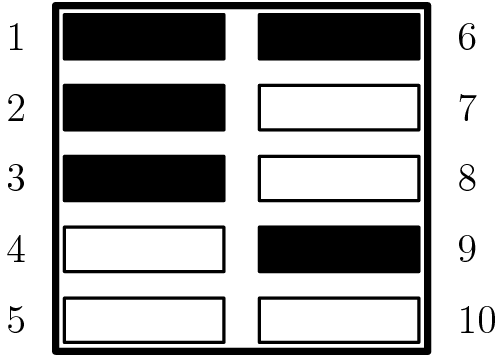
\includegraphics[width = 50.400000000000006mm]{img/fig0.png}
\end{center}